\section{Построение медианного МУ НОУ и оценка его результатов}

\begin{enumerate}
	\item *Представить ОУ~\ref{eq_iso_coc} в базисе, в котором 	неопределенность физических параметров представлена 	неопределенностью значений только матрицы состояния в	форме матричного компонента $\Delta A$;  
	\item Синтезировать закон медианного модального управления, базовый алгоритм которого дополняется контролем нормы  медианной составляющей интервальной матрицы  спроектированной системы с последующим вычислением оценки, вычислить матрицы $K_g$ и $K$. 
	Закон управления (ЗУ) вида $u(t) = K_g g(t)-K x(t)$ должен доставлять системе
	\begin{equation}
		\begin{cases}
			\dot x (t) = [F] x(t) + G g(t);\\
			y(t) = C x(t)
		\end{cases}
	\end{equation}
	образованной объединением НОУ и ЗУ равенство входа $g(t)$ и выхода $y(t)$ в неподвижном состоянии при номинальных значениях параметров с помощью:
	\begin{enumerate}
		\item матрицы $K_g$ прямой связи по входу $g(t)$;
		\item матрыцы $K$ обратной связи по состоянию $x(t)$
	\end{enumerate}
	распределение мод Баттерворта с характеристической частотой $\omega_0 = 3c^{-1}$, которая гарантирует достижение значение оценки относительной интервальности матрицы состояния системы $\delta_I = \cfrac{||\Delta F||}{||F_0||}$ не больше заданной $\delta_{IR}F = 0.02$; 
	\item Исследовать свойство робастности системы, полученной в п.1, с помощью метода В.Л. Харитонова;
	\item Моделирование полученной системы.
\end{enumerate}

\subsection{Получение ВМО НОУ с интервальными параметрами только матрицы состояния}

Модельная параметрическая неопределенность может быть представлена неопределенностью (интервальностью) задания только матрицы состояния объекта управления. Таким образом, объект управления с интервальными параметрами задается векторно-матричной моделью
\begin{equation}\label{eq:mmc}
	\begin{cases}
		\dot x (t) = [A] x(t) + B u(t);\\
		y(t) = C x(t)
	\end{cases}
\end{equation}
где $x \in R^n, u \in R^r, y \in R^m$ -- соответственно векторы состояния, управления и выхода ОУ; $[A], B, C$ -- интервальная матрица состояния, матрица управления и выхода, согласованные по размерности с переменными модели~\ref{eq:mmc}.

Из предыдущего утверждения становится очевидным, что матрицы ОУ полученные в п.5 не соответствуют предъявляемым к ним требованиям и нужно представить ОУ в форме~\ref{eq:mmc}.

Для этого нужно ОУ~\ref{eq_OU} привести к наблюдаемой (фробениусовой) канонической форме, тогда его матрицы примут вид
\begin{equation}\label{Aqn}
	A(q) =
	\begin{bmatrix}
	0 & - \cfrac{(1+q_4)(1+q_7)}{2(1+q_3)(1+q_6)} \\
	1 &-\cfrac{20(1+q_3)(1+q_7)+3.6(1+q_4)(1+q_6)}{12(1+q_3)(1+q_6)}
	\end{bmatrix}
\end{equation}
\begin{equation}\label{Bqn}
	B(q) =
	\begin{bmatrix}
		\cfrac{(1 + q_2)}{30(1+q_3)(1+q_6)}\\
		\cfrac{(1 + q_1)}{4(1+q_3)(1+q_6)} 
	\end{bmatrix}
\end{equation}

\begin{equation}\label{Cqn}
	C =
	\begin{bmatrix}
	0 & 1
	\end{bmatrix}
\end{equation}

Затем, так как полученные ОУ в каноническом наблюдаемом базисе не позволяет параметрическую неопределенность представить только в виде вариации $\Delta A$ матрицы
состояния, то на входе ОУ достаточно включить буферную систему~\cite{NSUsh}
\begin{equation}
	\begin{cases}
		{\dot x_B} (t) = A_B x_B(t) + B_B u_B(t) u(t);\\
		y(t) = C_B x_B(t)
	\end{cases}
\end{equation}
минимальной размерности $\dim x_B = \dim u = r = 1$ и ввести в рассмотрение составной вектор $\tilde{x} = col\{x, x_B\}$ и $\tilde{u} = col\{u, u_B\}$, получим систему
\begin{equation}
	\begin{cases}
		\tilde{\dot x} (t) = \tilde{A} \tilde{x}(t) + \tilde{B} \tilde{u}(t);\\
		y(t) = \tilde{C} \tilde{x}(t)
	\end{cases}
\end{equation}
где
\begin{align}
	\tilde{A} =
	\begin{bmatrix}
	 A(q) & B(q) C_B\\
	 0 & A_B
	\end{bmatrix};
	\tilde{B} = 
	\begin{bmatrix}
		0\\
		B_B
	\end{bmatrix};
	\tilde{C} = 
	\begin{bmatrix}
		C & 0
	\end{bmatrix}
\end{align}

Составим матрицы, при $A_B = 0, B_B = 1, C_B = 1$
\begin{align}
	\tilde{A} =&
	\begin{bmatrix}
		0 & - \cfrac{(1+q_4)(1+q_7)}{2(1+q_3)(1+q_6)} &	\cfrac{(1 + q_2)}{30(1+q_3)(1+q_6)}\\
		1 &-\cfrac{20(1+q_3)(1+q_7)+3.6(1+q_4)(1+q_6)}{12(1+q_3)(1+q_6)} & \cfrac{(1 + q_1)}{4(1+q_3)(1+q_6)} \\
		0&0&0
	\end{bmatrix};\\
	\tilde{B} =&
	\begin{bmatrix}
	0\\
	0\\
	1
	\end{bmatrix};
	\tilde{C} =
	\begin{bmatrix}
	0 & 1 & 0
	\end{bmatrix}
\end{align}

В соответствии с~\ref{interv},~\ref{midA},~\ref{widA}, запишем интервальную матрицу $[\tilde{A}] = \tilde{A}_0 + [\Delta A]$
\begin{align}
	[\tilde{A}] =
	\begin{bmatrix}
	    0&  - 0.6736111 &   0.0405093  \\
		1&  - 2.649537  &   0.3038194  \\
		0&    0        & 0 
	\end{bmatrix}
	+
	\begin{bmatrix}
		0&	[- 0.4514, 0.4514]	&[-0.02199, 0.02199] \\
		0&	[-1.7755, 1.7755]	&[-0.1649, 0.1649]\\
		0&0&0
	\end{bmatrix}
\end{align}

Таким образом, ОУ~\ref{eq:mmc} характеризуется параметрической неопределенностью только матрицы состояния.


\subsection{Синтез медианного МУ НОУ}

Порядок полученного в пункте 6.1 ОУ $\dim n = 3$, а ранг матрицы $\tilde{B}$ $rang \tilde{B} = 2$ и $rang \tilde{B} < \dim n$, следовательно возможно решение только неполной задачи обобщенного модального управления (ОМУ).

Агрегирование полученного ОУ и ЗУ
\begin{equation}
	u (t) = K_g g(t) - K x(t)
\end{equation}
образует систему 
\begin{equation}
	\begin{cases}
		\dot x (t) = [F] x(t) + G g(t);\\
		y(t) = C x(t)
	\end{cases}
\end{equation}
где 
\begin{equation}
	[F] = F_0 + \Delta F, \Delta F = \Delta A, G = B K_g.
\end{equation}

Найдем нормы медианной и интервальной составляющих матрицы $\tilde{A}$ (далее будем ее обозначать как $A$)
\begin{align}
    ||A_0|| = 2.92; ||\Delta A|| = 1.84
\end{align}

%Сформируем требования к показателям качества проектируемой системы: пусть $t_{n} \le 20c,  \sigma \le 50\%, \delta_{IR} F = 0.02$.

Выберем наблюдаемую пару матрицу модальной модели ($\Lambda$, H). Назначим матрицу $\Lambda$, соответствующую круговому распределению мод с характеристической частотой $\omega_0$ такой, что $||\Lambda|| \ge \omega_0$ и
\begin{equation}
	\Lambda = \arg\{||\Lambda|| \ge \cfrac{||\Delta A||}{\delta_{I} F} \& \sigma\{\Lambda\} = \sigma\{F\} \}
\end{equation}

Значение характеристической частоты $\omega_0$ определяется в силу технических требований к проектируемой системе из условия
\begin{equation}
	\omega_0 = max \{\omega_0 <= \cfrac{6}{2} = 3c^{-1}; \omega_0 <= \cfrac{||\Delta A||}{\delta_{IR}} = \cfrac{2.92}{0.02} =  146c^{-1}\} = 146 c^{-1}
\end{equation}

Найдем матрицу $\Lambda$
\begin{align}
	\Lambda = \omega_0 
	\begin{bmatrix}
	  - 0.0260481&    0.   &        0.\\         
		0.    &     - 0.0011358 &   0.  \\       
		0.   &        0.      &   - 12.057286 	
	\end{bmatrix}
	=\\=
	\begin{bmatrix}
	  - 3.8030252   & 0.       &    0.\\         
		0.        & - 0.1658288&    0.  \\       
		0.        &   0.    &     - 1760.3637 
	\end{bmatrix}
\end{align}
\begin{equation}
	||\Lambda|| = 1760.36
\end{equation}

Модификация матрицы $H$ осуществляется в силу алгоритмов линейного программирования,
таких как алгоритм Нелдера–Мида. В итоге матрица $M$ ищется с помощью итерационной процедуры, приводящей к выполнению условия:
\begin{equation}
	M = \arg \min_H \{C\{M(H)\} : M \Lambda - A M = - B H : \Lambda = fix, H = var\}
\end{equation}
где начальное значение $H = \begin{bmatrix}1&1&1\end{bmatrix}$.

Выполнение этой процедуры дает следующие реализации матриц 
\begin{equation}
	H = 
	\begin{bmatrix}
	 - 0.0053596  &  0.000099  &  2.3063721 
	\end{bmatrix}
\end{equation}
\begin{equation}
	M = 
	\begin{bmatrix}
	    0.00007 &  - 0.0002374 & - 3.024D-08\\  
		0.0003105 & - 0.0000225 & - 0.0000002 \\ 
		- 0.0014093 &   0.0005972 &   0.0013102 
	\end{bmatrix}
\end{equation}

Наименьшее число обусловленностей, которой удалось получить при задании различных комбинация матриц $\Lambda$
\begin{equation}
	C\{M\} = 9.45
\end{equation}

Произведем расчет матриц регулятора. Матрицы ОС $K$ имеет реализацию
\begin{equation}
	K = H M^{-1} = 
	\begin{bmatrix}
	3754.6837 &   7131.9983   & 1761.6831
	\end{bmatrix}
\end{equation}

Матрица прямых связей $K_g$
\begin{equation}
	K_g = -(C * F^(-1) * B)^(-1) =
	\begin{bmatrix}
		27422.098 
	\end{bmatrix}
\end{equation}

Вычислим матрицу замкнутой системы $F$ 
\begin{equation}
	F0 = A0 - B K =
	\begin{bmatrix}
	    0.&        - 0.6736111 &   0.0405093  \\
		1. &        - 2.649537  &   0.3038194  \\
		- 3754.6837 & - 7131.9983 & - 1762.6831 
	\end{bmatrix}
\end{equation}

Вычислим полученную оценку относительной интервальности матрицы~$F$
\begin{equation}
	\delta_{IF} = \cfrac{||\Delta A||}{||F0||} = \cfrac{1.84}{8250.46} = 0.0002229 < 0.02
\end{equation}

\subsection{Исследование свойства робастности системы}
Представим матрицу $F$ в интервальном виде
\begin{equation}
	\Delta F = \Delta A = 
	\begin{bmatrix}
		0  &[- 0.45138, 0.45138] &  [- 0.02199, 0.02199]\\  
		0  &[- 1.7754, 1.7754] &   [- 0.16493, 0.16493]  \\
		0  &  0     &      0         
	\end{bmatrix}
\end{equation}


\begin{equation}
	[F] = 
	\begin{bmatrix}
	0 &        [- 1.125, - 0.2222222] &       [0.0185185, 0.0625]  \\ 
	1  &       [- 4.425, - 0.8740741]  &      [0.1388889, 0.46875]  \\
	- 3754.6837 & - 7131.9983&  - 1762.6831  

	\end{bmatrix}
\end{equation}

Найдем характеристический полином $D(\lambda, q)$ матрицы $F(q)$
\begin{equation}\label{char}
	D(\lambda, q) = det(\lambda I -F(q)) = [a_0] \lambda^3 + [a_1] \lambda^2 + [a_2] \lambda + [a_3]
\end{equation}
где $[a_n]$~-- интервальный параметр вида $[\underline{a_n}, \overline{a_n}]$.

По теореме В. Л. Харитонова, чтобы интервальный характеристический полином~\ref{char}
был гурвицевым необходимо и достаточно, чтобы были гурвицевыми четыре его угловые версии, имеющие представления
\begin{align}
	&D(\lambda) = \underline{a_3} + \underline{a_2} \lambda + \overline{a_1} \lambda^2 + \overline{a_0} \lambda^3\\
	&D(\lambda) = \overline{a_3} + \underline{a_2} \lambda + \underline{a_1} \lambda^2 + \overline{a_0} \lambda^3\\
	&D(\lambda) = \overline{a_3} + \overline{a_2} \lambda + \underline{a_1} \lambda^2 + \underline{a_0} \lambda^3\\
	&D(\lambda) = \underline{a_3} + \overline{a_2} \lambda + \overline{a_1} \lambda^2 + \underline{a_0} \lambda^3
\end{align}

Найдем интервальные коэффициенты ИХП~\ref{char} методом Крамера
\begin{align}
	&[a_0] = [1,1];\\
	&[a_1] = -tr[F] = [178579.4658, 178583.0167];\\
	&[a_2] = [M_{11}] + [M_{22}] = [136062041.6772, 136697531.9607];\\
	&[a_3] = -det[F] = [43933256.2435, 156394735.1753]
\end{align}

Тогда полиномы запишутся, как 
\begin{align}
	&D(\lambda) = 43933256.2435 + 136062041.6772 \lambda + 178583.0167 \lambda^2 + \lambda^3\\
	&D(\lambda) = 156394735.1753 + 136062041.6772 \lambda + 178579.4658 \lambda^2 + \lambda^3\\
	&D(\lambda) = 156394735.1753 + 136697531.9607 \lambda + 178579.4658 \lambda^2 + \lambda^3\\
	&D(\lambda) = 43933256.2435 + 136697531.9607 \lambda + 178583.0167 \lambda^2 + \lambda^3
\end{align}

Все полиномы В. Л. Харитонова гурвицевы, следовательно, гурвицев ИХП $[D(\lambda)]$. Система робастно устойчива.

\subsection{Моделирование полученной системы}

\begin{figure}[h!]
	\centering
	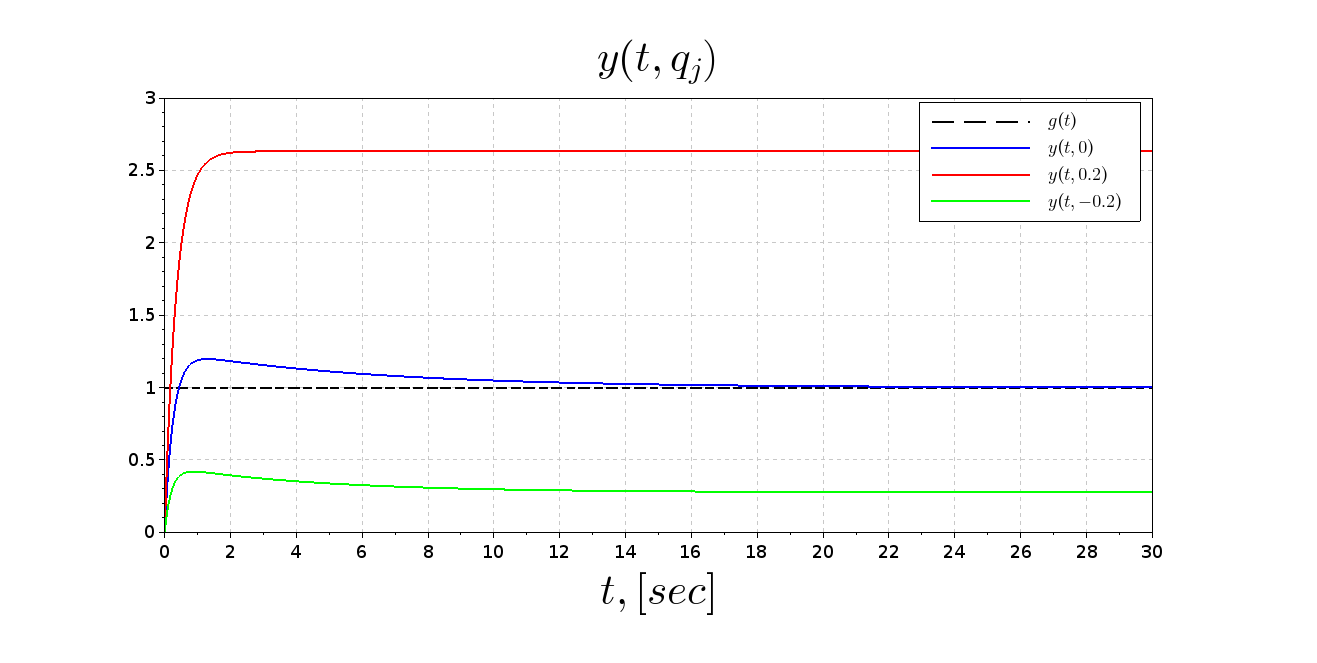
\includegraphics[width=1\textwidth]{problem6_res.png}
	\caption{Результаты моделирования ММУ при $q = [\underline{-0.2}, \overline{0.2}]$}
	\label{}
\end{figure}
\newpage



\begin{figure}[h!]
	\centering
	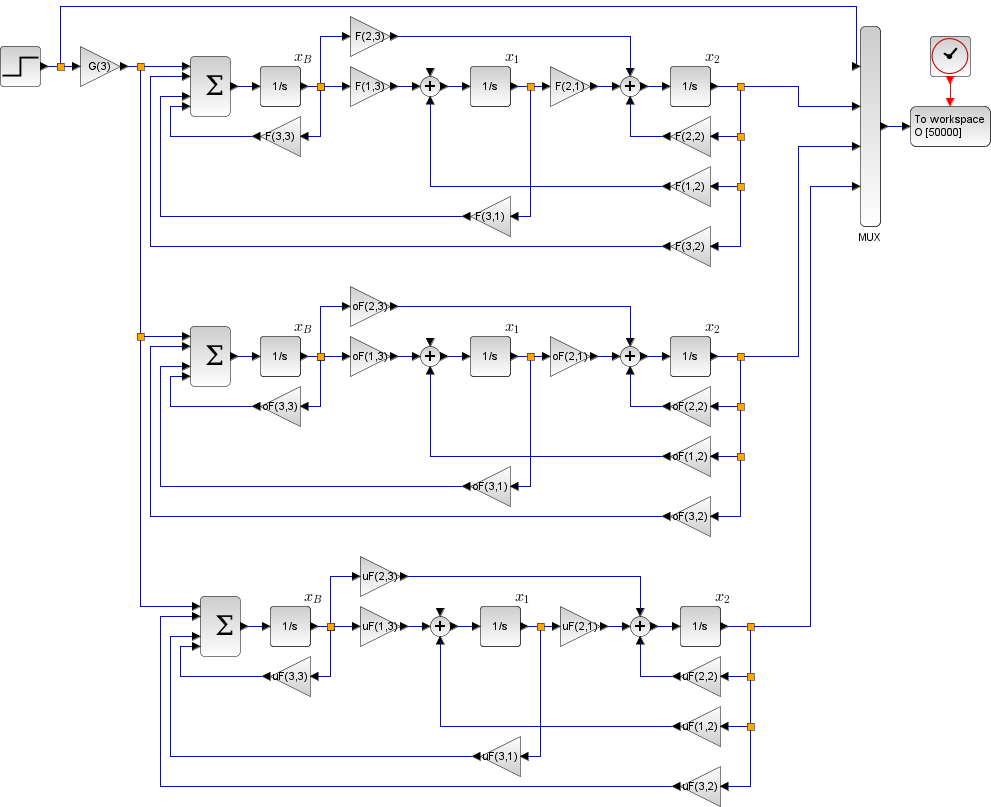
\includegraphics[width=1\textwidth]{problem6.png}
	\caption{Схема моделирования ММУ}
	\label{}
\end{figure}


\newpage